\chapter{Theoretical Framework}

This chapter reviews the theoretical base to model ultrashort-pulse propagation in fibers. Spectral and time broadening are fundamental aspects of nonlinear fiber optics. Understanding their basis and how they affect the propagation of an electromagnetic wave is an essential factor to both develop the code and test its effectiveness. Providing an overview of the equations describing the light propagation in a dispersive, nonlinear medium gives the principles to see what is solved with the back-end code at further stages in this thesis project.

\section{Eigenvalue problem}

\subsection{Planar Waveguide}



\begin{figure}[label={fig_planarwave}, caption={Sketch of a planar waveguide.}]
  %  \caption*{Source: Some Source}
        \centering  
        \tikzset{every picture/.style={line width=0.75pt}} %set default line width to 0.75pt   
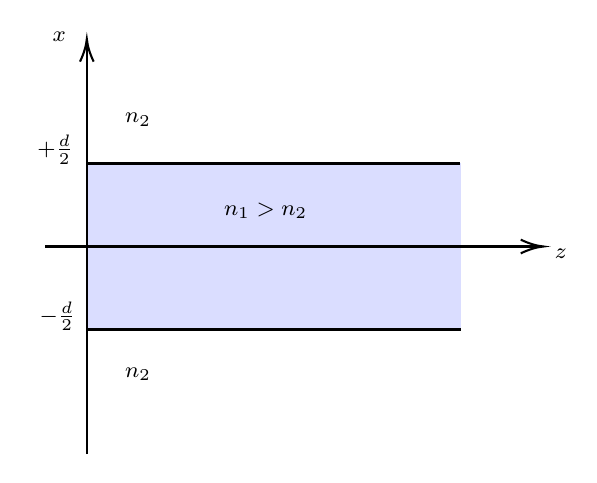
\begin{tikzpicture}[x=0.75pt,y=0.75pt,yscale=-1,xscale=1]
%uncomment if require: \path (0,310); %set diagram left start at 0, and has height of 310

%Shape: Rectangle [id:dp439999456910388] 
\draw  [draw opacity=0][fill={rgb, 255:red, 218; green, 221; blue, 255 }  ,fill opacity=1 ] (100,80) -- (280.5,80) -- (280.5,160) -- (100,160) -- cycle ;
%Shape: Boxed Line [id:dp5082075899729874] 
\draw    (80,120) -- (318,120) ;
\draw [shift={(320,120)}, rotate = 180] [color={rgb, 255:red, 0; green, 0; blue, 0 }  ][line width=0.75]    (10.93,-3.29) .. controls (6.95,-1.4) and (3.31,-0.3) .. (0,0) .. controls (3.31,0.3) and (6.95,1.4) .. (10.93,3.29)   ;
%Shape: Boxed Line [id:dp5101173446407539] 
\draw    (100,220) -- (100,22) ;
\draw [shift={(100,20)}, rotate = 450] [color={rgb, 255:red, 0; green, 0; blue, 0 }  ][line width=0.75]    (10.93,-3.29) .. controls (6.95,-1.4) and (3.31,-0.3) .. (0,0) .. controls (3.31,0.3) and (6.95,1.4) .. (10.93,3.29)   ;
%Shape: Boxed Line [id:dp2709424820833741] 
\draw    (100.5,160) -- (280.5,160) ;
%Shape: Boxed Line [id:dp10541842748284669] 
\draw    (100,80) -- (280,80) ;


% Text Node
\draw (74.67,64.73) node [anchor=north west][inner sep=0.75pt]  [font=\footnotesize]  {$+\frac{d}{2}$};
% Text Node
\draw (72,145.07) node [anchor=north west][inner sep=0.75pt]  [font=\footnotesize]  {$\ -\frac{d}{2}$};
% Text Node
\draw (164.67,97.73) node [anchor=north west][inner sep=0.75pt]  [font=\footnotesize]  {$n_{1}  >n_{2}$};
% Text Node
\draw (117,177.07) node [anchor=north west][inner sep=0.75pt]  [font=\footnotesize]  {$n_{2}$};
% Text Node
\draw (117,54.4) node [anchor=north west][inner sep=0.75pt]  [font=\footnotesize]  {$n_{2}$};
% Text Node
\draw (324,119.73) node [anchor=north west][inner sep=0.75pt]  [font=\footnotesize]  {$z$};
% Text Node
\draw (82,15.07) node [anchor=north west][inner sep=0.75pt]  [font=\footnotesize]  {$x$};


\end{tikzpicture}

\end{figure}
  
Figure \ref{fig_planarwave} shows a planar waveguide consisting of two materials with refractive indices $n_1$ for the core and $n_2$ for the cladding. This waveguide is infinite in the y-direction, has a thickness $d$ (which satisfies that $d >> \lambda$), and fulfills the total internal reflection condition at the boundary.  Its transverse propagation constant is


            \begin{equation}
                h=\sqrt{k_0^2n_1^2-\beta^2},
                \label{eq_h}
            \end{equation}
 where $\beta$ and $h$ are for the core region. For the cladding region, we have the longitudinal propagation constant $\kappa$

             \begin{equation}
                \kappa=\sqrt{\beta^2-k_0^2n_2^2}.
                \label{gam}
            \end{equation}
 
 Here $k_0 = \omega_0/c$ is the wavenumber in vacuum.



We can include U, W, and V

            \begin{equation}
                U^2+W^2 = V^2 = k_0^2a^2(n_1^2-n_2^2) \
                \begin{cases}
                    U = a \times h \\
                    W = a \times \kappa
                \end{cases} 
                \label{Normv},
            \end{equation}
where V is the so-called waveguide parameter or normalized frequency. 
The TE mode is then given by 
         
            
            \begin{equation}
            \textbf{TE mode} \ \ W=
                \begin{cases}
                    U \tan(U) & \text{even mode}\\
                    -U cotan(U) & \text{odd mode}
                \end{cases}
                \label{Temode}
            \end{equation}

We can solve the eigenvalue problem graphically by plotting W as a function of U [Joly's lecture]. Figure \ref{fig:eigen1} shows this approach where the circle has a radius of V.


\begin{figure}[label={fig:eigen1}, caption={Visualization of the graphic solution of the eigenvalue problem. Taken from \cite{herokuapp}}]
  %  \caption*{Source: Some Source}
	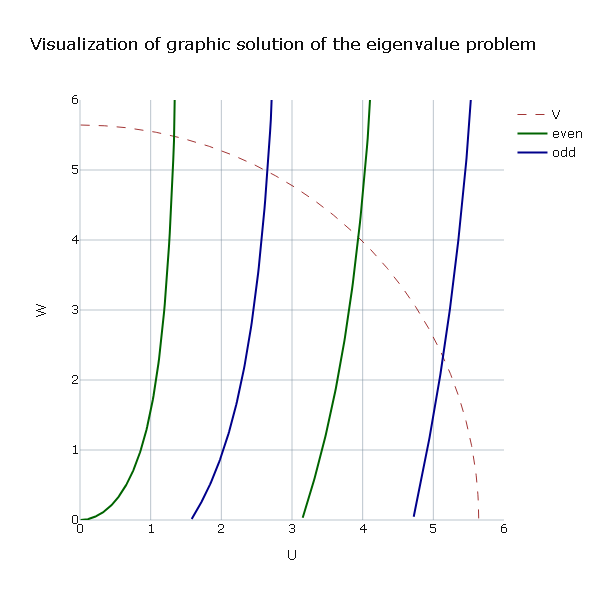
\includegraphics[width=.6\textwidth]{figures/chap2/Eigenvalue.png} 
\end{figure}

We created a code at the Max-Plank institute \cite{gitmax} to show the students how a change of parameters can affect the plot and, thus, the solutions of the eigenvalue problem. This web tool aims to help the students understanding this problem, and figure \ref{fig:planarp}  shows the interface. The code is written in Python and the Web interface made with Dash/Plotly.  

\begin{figure}[label={fig:planarp}, caption={\href{https://fiber-mode-app.herokuapp.com/apps/dash_plot}{Heroku app} for the planar waveguide.}]
  %  \caption*{Source: Some Source}
	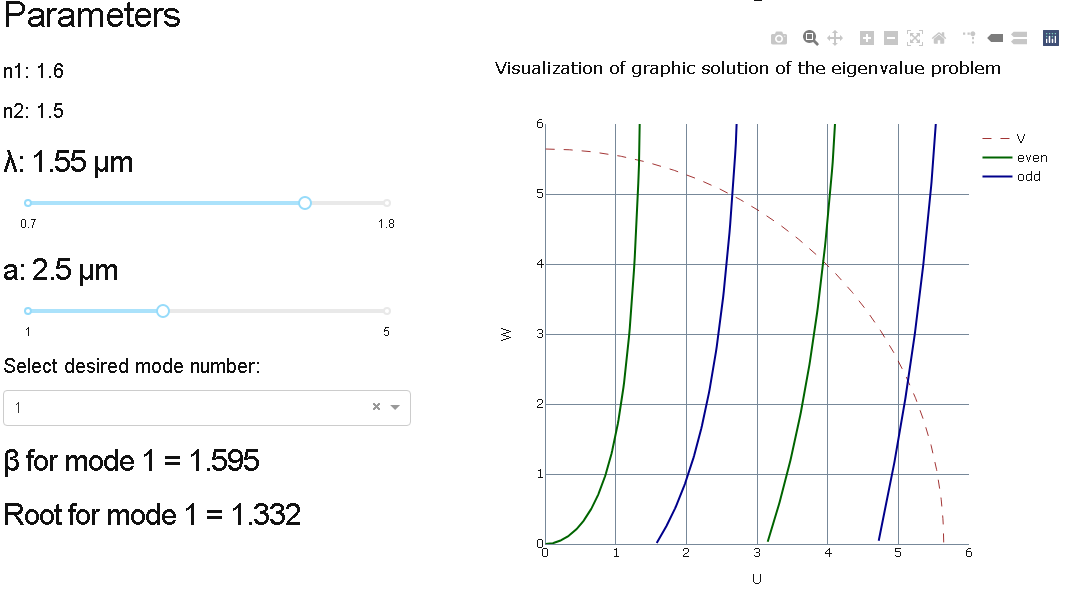
\includegraphics[width=.8\textwidth]{figures/chap2/planarpage.png} 
\end{figure}


Heroku is a web that supports programming languages like Java, Node.js, Python, among others \cite{heorku}. The codes for the planar waveguide and the optical fiber were deployed using its free service.

\subsection{Optical Fiber}

The code can also solve the problem for the optical fiber, and the students can change some more parameters like cladding and core material, see the Poynting vector or some of the cuts of the field. Figures \ref{fig:fibre1} and \ref{fig:fibre2} show this web. 


The refractive index of a material can be approximated by 
\begin{equation}
    n^2 (\omega) = 1 + \sum_{j=1}^{m} \frac{B_j\omega^2_j}{\omega^2_j - \omega^2} 
    \label{eq_ene}
\end{equation}
called the Sellmeier equation. Here $\omega_j$ is the resonance frequency and $B_j$ the strength of it \citep{AgrawalBook}. This allowed to add the different materials to de code an can be changed by selecting the material in the dropwdowns for the core and the cladding of the fiber.


\begin{figure}[label={fig:fibre1}, caption={\href{https://fiber-mode-app.herokuapp.com/apps/results}{Heroku app} for the optical fiber (1).}]
  %  \caption*{Source: Some Source}
	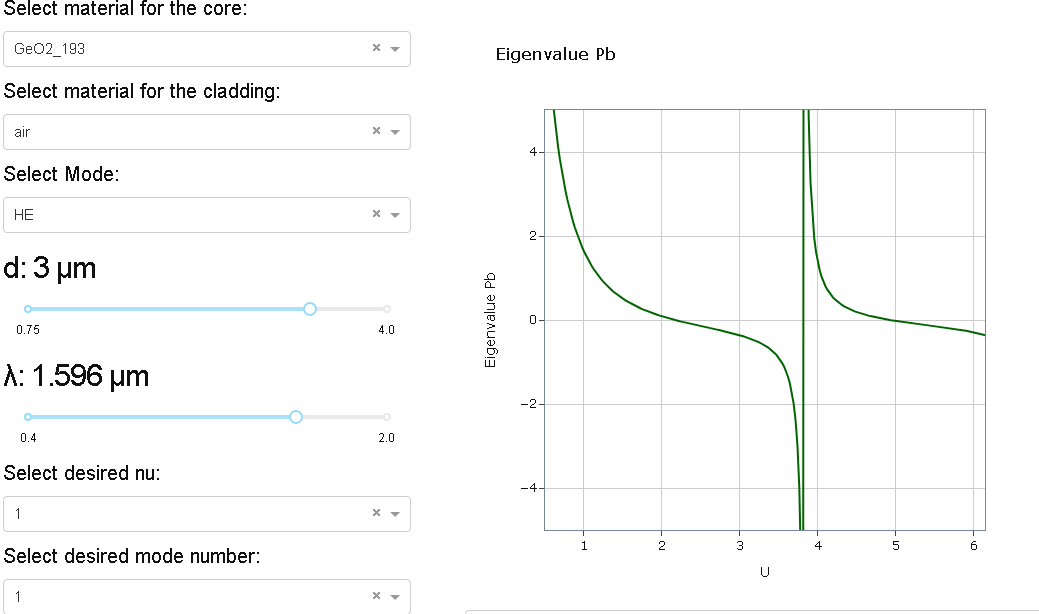
\includegraphics[width=.8\textwidth]{figures/chap2/fibre1.PNG} 
\end{figure}

\begin{figure}[label={fig:fibre2}, caption={\href{https://fiber-mode-app.herokuapp.com/apps/results}{Heroku app} for the optical fiber (2).}]
  %  \caption*{Source: Some Source}
	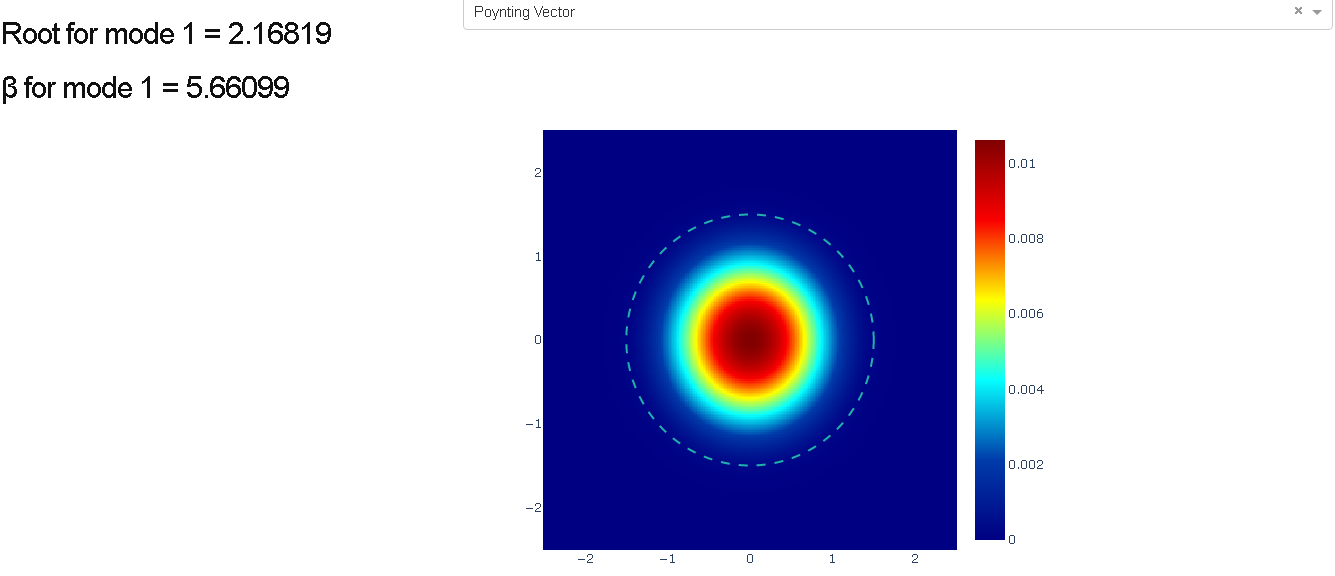
\includegraphics[width=.8\textwidth]{figures/chap2/fibre2.PNG} 
\end{figure}


   


\section{Pulse propagation in fibers}

Loss and dispersion originated by interactions of the electromagnetic field with the atoms of the medium, and frequency dependence of the refractive index affect the propagation of an electromagnetic wave through this medium \citep{dudley_taylor_2010}. Shape and spectrum of short pulses with widths between approx. 10ns and 10fs propagating in a fiber are affected by nonlinear and dispersive effects \citep{AgrawalBook}.  

    \subsection{Pulse evolution inside a single-mode fiber:}
        The slowly varying amplitude \emph{A(z,t)} can be described by the equation:
        \begin{equation}\label{eq_a}
        \begin{split}
\frac{\partial A}{\partial z}&= \overbrace{-\frac{\alpha}{2} - \beta_1\frac{\partial A}{\partial t} - \frac{i \beta_2}{2} \frac{\partial^2 A}{\partial t^2} +\frac{\beta_3}{6} \frac{\partial^3 A}{\partial t^3}}^{\mathbf{linear \ effects}}\\  
            & +\underbrace{i \gamma \left( 1 + \frac{i}{\omega_0} \frac{\partial}{\partial t} \right) \left( A(z,t) \int_{-\infty}^{\infty} R(t') \left|A(z, t-t') \right|^2 \ dt'  \right)}_{\mathbf{nonlinear \ effects}}
        \end{split}
        \end{equation}
    %[A] = sqrt(W)
    where: 
    \begin{itemize}
        \item \textbf{t} is the time variable [s]
        \item \textbf{z} is the space variable [m]
        \item $\mathbf{\alpha}$ is the attenuation coefficient [1/m]
        \item $\mathbf{\beta_n}$ are propagation constant coefficients $[s^n/m]$
        \item $\mathbf{\gamma}$ is the nonlinear parameter [1/Wm]
        
            \begin{equation}
                \gamma = \frac{n_2 \omega_0}{c A_{eff}},
                \label{eq_gamma}
            \end{equation}
        with $\mathbf{n_2} \quad [m^2/W]$ which is the nonlinear refractive index, and $A_{eff} \quad [m^2]$ that  is the  effective core area.
        %or  n2 is the nonlinear-index coefficient. 
        \item \textbf{R(t)} [1/s] is the response function that includes electronic and vibrational contributions and is approximated by 
        
        \begin{equation}\label{eq_rt}
            R(t) = (1- f_R)\delta(t) + f_R h_R(t),
        \end{equation}
        where $f_R$ and $h_R(t)$ are the fractional contribution of the delayed Raman response and the Raman response function, respectively. Conforming to \cite{dudley_taylor_2010}, 
        \begin{equation}\label{eq_hr}
            h_R(t) = \frac{\tau^2_1+\tau^2_2}{\tau_1\tau^2_2} exp(-t/\tau_2)sin(t/\tau_1)\Theta(t),
        \end{equation}
        here $\delta(t)$ and $\Theta(t)$ are the Delta Dirac and the Heaviside step functions, respectively; $f_R = 0.18$,  $\tau_1 =12.2 fs$, and $\tau_2 = 32 fs$.
         
         
        \item $\omega_0$  is the center angular frequency
    
    \end{itemize}
   
    One can asume that the evolution of the envelope pulse is slow, and remembering that the group velocity is defined by 
    
    \begin{equation}\label{eq_vg}
        v_g \equiv \frac{1}{\beta_1}, 
    \end{equation}
    the pulse can be moved at the group velocity using the reference frame 
    \begin{equation}\label{eq_t}
        T = t - \frac{z}{v_g}. 
    \end{equation}
    
    Thus, equation \eqref{eq_a} can be defined as 
    
    \begin{equation}\label{eq_b}
        \frac{\partial A}{\partial z}=-\frac{\alpha}{2} - \frac{i \beta_2}{2} \frac{\partial^2 A}{\partial T^2} +\frac{\beta_3}{6} \frac{\partial^3 A}{\partial T^3} +i \gamma   \left(A\left|A\right|^2+ \frac{i}{\omega_0} \frac{\partial}{\partial T} (A\left|A \right|^2)- A \ T_R \frac{\partial \left|A \right|^2}{\partial T} \right),
        \end{equation}
    where the first moment of the nonlinear (Raman) response is
    \begin{equation}\label{eq_TR}
        T_R = f_R\int_{0}^{\infty} t \ h_R(t) \ dt.
    \end{equation}

        
    \subsection{NLSE}
        According to \citep{AgrawalBook}, the equation  \eqref{eq_b} for the slowly varying envelope can be simplified for pulses of width $T_0 > 5 ps$ to
        \begin{equation}
                \frac{\partial A}{\partial z} = \frac{\alpha}{2}A-j \frac{\beta_2}{2}\frac{\partial^2A}{\partial T^2}+j\gamma|A|^2 A,
                \label{eq_nlse}
            \end{equation}
            \ \\
       It is noteworthy that the contribution of the third-dispersion term should be considered if $\beta_2 \approx 0$ (zero-dispersion region). Equation \eqref{eq_nlse} is known as the nonlinear Schrödinger equation (NLSE).

           Following the convention used in \cite{AgrawalBook}, \cite{dudley_taylor_2010} , the continuous inverse Fourier transform of the slowly varying function of z is
        
        \begin{equation}\label{eq_acft}
            A(z,t) = \frac{1}{2*\pi} \int_{-\infty}^{\infty} \tilde{A}(z,\omega-\omega_0)\exp{[-i(\omega-\omega_0)t]} \ d\omega \ .
        \end{equation}
        
        
        The FFT is an algorithm capable of calculating the discrete Fourier transform faster \citep{Lynch2018}. The definition of \href{https://numpy.org/doc/stable/index.html}{Numpy} of the inverse DFT as \cite{dft} says is 
        \begin{equation}\label{eq_dft}
            a_n = \frac{1}{n}\sum_{k=0}^{n-1} A_k \ exp\left\{ 2\pi i \frac{mk}{n} \right\} \qquad m = 0,...,n-1,
        \end{equation}

        then, it follows
        \begin{equation} \label{eq_deffft}
                A(z,T) = FFT \left[ \tilde{A}(z,\omega) \right].
            \end{equation}
            
            
        \subsection{Dispersion}
    The frequency dependency of the refractive index can lead to different speeds of propagation from different wavelengths of pulses in a fiber, which causes a broadening of the pulse in the time domain. This effect can limit the transmission of information and generate effects like inter symbol interference.  So, one can call chromatic dispersion the delay between several spectral components of a traveling pulse, i.e., there are different group velocities for the diverse components propagating in the fiber  \citep{Udayakumar2013ChromaticDC}. This delay depends on the waveguide (e.g., core radius) and material (e.g., the difference between core and cladding indices) contributions \citep{dudley_taylor_2010}. 
    
    The Taylor series expansion of the propagation constant 
    \begin{equation}
         \beta(\omega) = n (\omega)\frac{\omega}{c} = \beta_0 + \beta_1(\omega-\omega_0) \frac{1}{2}\beta_2(\omega-\omega_0)^2+...\, 
         \label{eq_betas}
    \end{equation}
    with 
    \begin{equation}
        \beta_m = \frac{d^m\beta}{d\omega^2}_{\omega = \omega_0} \qquad (m = 0,1,2,...),
        \label{eq_dbeta}
    \end{equation}
    
    
    defines the Group Velocity Dispersion (GVD) parameter $\beta_2$  and higher-order dispersion terms.  $\beta_2$ is also related to the dispersion parameter D by
    \begin{equation}
        D = \frac{d\beta_1}{d\lambda} = \frac{2\pi c}{\lambda^2}\beta_2 \quad [\frac{ps}{nm \ km}] \ .
        \label{eq_Ds}
    \end{equation}
    
    Depending on the value of the GVD parameter shows the fiber a normal dispersion ($\beta_2 > 0$), or it is in the anomalous dispersion regime ($\beta_2 < 0$).
    
    Linear solitons can reduce this effect, even though there are several methods to compensate chromatic dispersion, as \cite{AgrawalBook}, \cite{dudley_taylor_2010},  and \citep{Udayakumar2013ChromaticDC} explain. Dispersion compensating fiber (DCF), Fiber Bragg Grating (FBG), and Optical Phase Conjugator (OPC) are some of the methods used.
    
   

\subsection{Nonlinear Effects}

    Nonlinearities can be effects such as third-harmonic generation, four-wave mixing (FWM). The Kerr nonlinearity $n = n(P_{opt})$
    can lead to a time-dependent phase delay of the pulse itself, known as self-phase modulation, to a co-propagating pulse, known as cross-phase modulation (XPM), or the formation of a fourth component through up to three light waves with different frequencies (FMW ) \cite{rein}. The refractive index is written as
    
    
    \begin{equation}
        \tilde{n} (\omega, \left| E \right|^2) = \overbrace{n(\omega)}^{linear \ part \ Eq. \ \eqref{eq_ene}} + \underbrace{ n_2 \left| E \right|^2}_{nonlinear part},
    \end{equation} 
   
   where $n_2 = \frac{3}{8n}Re\left\{ \chi^{(3)}_{\chi \chi \chi}\right\}$ and $\chi^{(3)}$ is the third-order susceptibility.
   
   \subsubsection{Stimulated Inelastic Scattering}
    A further aspect of the nonlinear effects is the stimulated inelastic scattering. These effects are the stimulated Raman and Brillouin scattering (SRS and SBS, respectively). Vibrations of the molecular bonds of the medium interact with the injected pulse, which can lead to an amplification of the "Stokes wave" through a scattering power transfer by the molecular vibrations \cite{rein}. A main difference is that SRS and SBS involve then optical and acoustic phonons, respectively \cite{AgrawalBook}.
   
        \section{Solution of the NLSE}
    
        It is common to solve the nonlinear differential equations \eqref{eq_b} and \eqref{eq_nlse} by a numerical method instead of analytical methods like \citep{Mihalache_1993}.  


    \subsection{Step-Doubling Technique}
         \citep{dudley_taylor_2010}uses an adaptative algorithm to propagate the solution of the NLSE, having two steps of calculation and a longer one equivalent starting at the same point. Therefore, they estimate the error through the differences between computations to converge more quickly. In \citep{gitdud}  is presented a Matlab-based code using this step-doubling technique. 
         
    \subsection{Split-Step Fourier Method}

    In this thesis, the split-step Fourier method (SSFM) was the numerical method selected to solve the NLSE. \citep{AgrawalBook}, \citep{sinkin}, \citep{robust},  and \citep{HohageSchmidt2002} show different approaches and points of view of this method.  \citep{robust} gives a robust SSFM,  \citep{sinkin} explains how to select optimized step sizes depending on the accuracy or effect desired to inspect with the SSFM, and  \citep{HohageSchmidt2002} offers a comparison between the different kinds of SSFM (). 
    
    
 
%Write eq for propagation and explain LD vs LNL Bereiche ->  GVD only -> U(0,T) Gauss- und Sech-Pulse -> wie wird das Programm durchgeführt? Ergebnisse mithilfe Matplotlibs, und Darstelung in einer Web-App 